\section{Results: Survey}
\label{section:Results_Survey}

\subsection{Population Selection}
We initially had two sources for our Experienced Drools users to send our survey to.
From LinkedIn we selected users who were at one degree of separation from us and listed Drools in their skills.
From StackOverflow we selected users who had asked or answered questions about Drools.

As in these two websites the users do not tend to list their contact details, some investigation was required.
From the initial selection, whose size we did not record we harvested email accounts, and failing that twitter accounts.

A few days into our survey we read a paper that described the use of academic papers as a population of expertise.
We used Google Scholar to look up Drools papers from the previous 2 years.
After skimming the papers to ensure that it was specifically about or using the Drools language we harvested emails

On the second and fourth day of the survey two subjects forwarded the weblink to the survey to mailing lists.
One, a developer from the core Drools team, sent it to a list of known Drools consultants.
The other sent it internally in his company.
both the subjects who sent the survey to their mailing list forwarded links to version C of the survey.

We had created 4 versions of the questionnaires to a combat single source bias.
We distributed the surveys to the subjects harvested from LinkedIn and StackOverflow evenly.
Because of the overrepresentation of Survey C, we distributed the subjects harvested from academic papers evenly over Surveys A, B and D.

The collection result can be seen in figure \ref{fig:Survey_participants}.
What we see here is that the method of collection did not have much of an impact on return rates.
whilst StackOverflow had a higher rate, the number of people contacted was so small that a small addition of respondents has an outsized effect on the proportion.

The first three pie charts represents the collection methods over which we had control.
These three represented 24 of our 30 completed questionnaires.
The last pie chart represents 6 completed and 4 partially completed questionnaires, that were returned from the surveys sent on by our initial participants.
We do not know the size of the starting population of these lists. 
Thus this pie chart only shows the ratio of partial to completed results.

In summary, a survey reached known 154 participants, of which 24 completed it, for a Response Rate of 15.5\%.
In addition, an unknown amount of participants were reached through mailing lists, returning a further 6 completed surveys.

\subsection{Participant Demography}

Responses came from around the world.
Figure \ref{fig:Survey_locations} shows the location of the respondents were concentrated in Europe, the exceptions being the USA, Israel, and Singapore.
Italy and the Netherlands provided the largest number of responses, with 7 and 5 respectively.

\begin{figure}[H]
    \centering
    \fbox{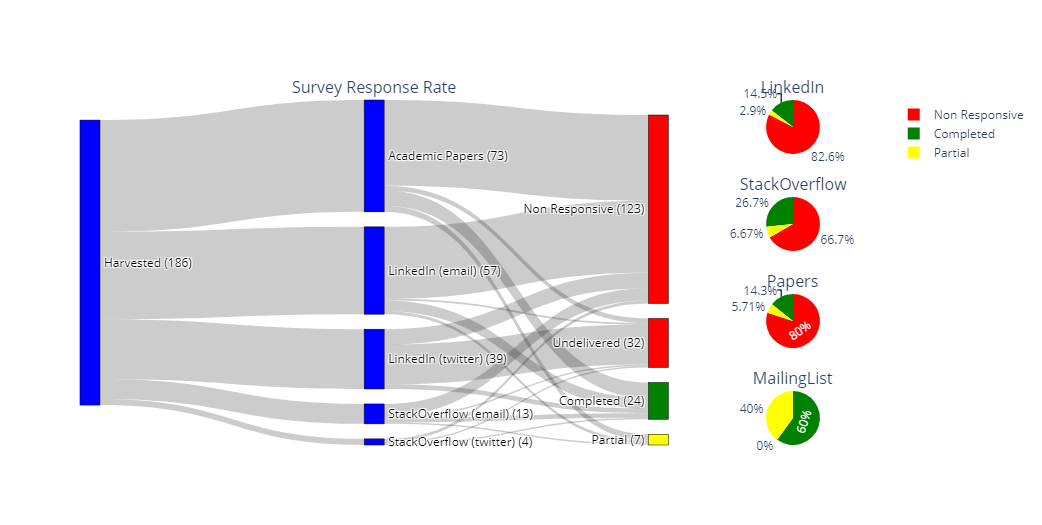
\includegraphics[width=0.95\textwidth]{Sections/images/survey_participants.png}}
    \caption{Survey participants}
    \label{fig:Survey_participants}
\end{figure}

\begin{figure}[H]
    \centering
    \fbox{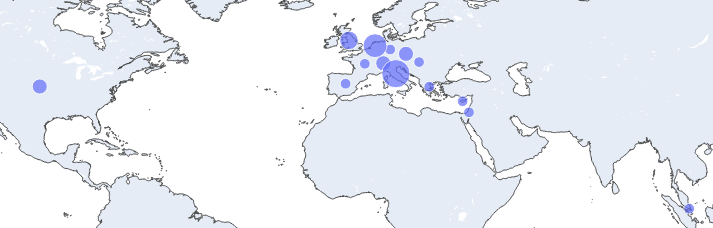
\includegraphics[width=0.95\textwidth]{Sections/images/survey_locations.png}}
    \caption{Survey locations}
    \label{fig:Survey_locations}
\end{figure}

\begin{figure}[H]
    \begin{subfigure}{.33\textwidth}
      \centering
      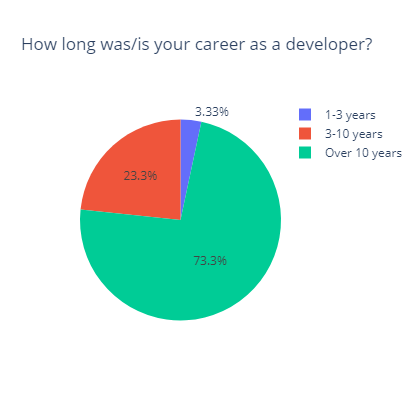
\includegraphics[width=.95\linewidth]{Sections/images/pie_experiencer.png}
      \caption{SE experience}
      \label{fig:sfig1}
    \end{subfigure}%
    \begin{subfigure}{.33\textwidth}
      \centering
      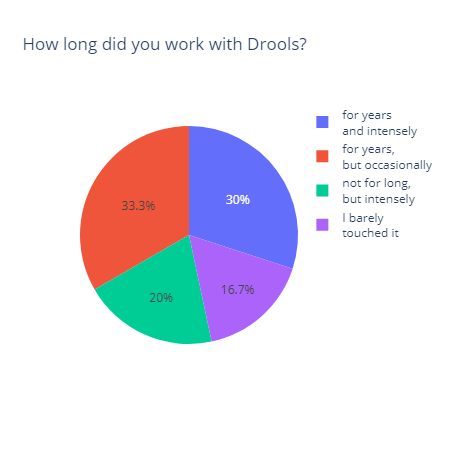
\includegraphics[width=.95\linewidth]{Sections/images/pie_droolsExperience.png}
      \caption{Drools experience}
      \label{fig:sfig2}
    \end{subfigure}
    \begin{subfigure}{.33\textwidth}
        \centering
        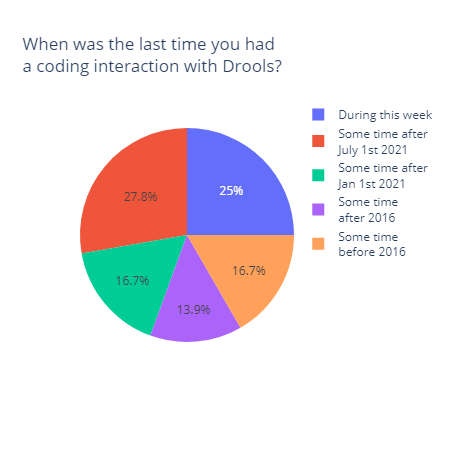
\includegraphics[width=.95\linewidth]{Sections/images/pie_recentusage.png}
        \caption{Recent use}
        \label{fig:sfig3}
      \end{subfigure}
    \caption{Subject experience}
    \label{fig:subject_experience}
\end{figure}

The experience of our subjects was quite high.
As can be seen in \ref{fig:sfig1}, most of our subjects have over 10 years programming experience.
17\% of our recipients had a low experience of Drools, and 30\% were very experienced, as shown in figure \ref{fig:sfig2}.
Figure \ref{fig:sfig3} reports that over half of our recipients have used Drools in the previous 6 weeks with only 17\% not having used Drools for more than 5 years.

Half of our subjects reported only ever using one editor for Drools, with the slight majority of those only using Eclipse.
Eclipse also had the most instances of reporting of having been used, out of the 55 instances of editors reported as being used, 20 of those were Eclipse.
There was a, to us, surprising diversity of tools being used.
The purpose of this section was to be able to calibrate responses against exposure to IDEs with greater Drools Support.
The wide diversity of editor usage and high incidence of multiple editor usage means that these answers are not suitable for use in the sub-categorisation of responses. 
The distribution of usage is shown in figure \ref{fig:editorUsage}.

\begin{figure}[h]
    \centering
    \fbox{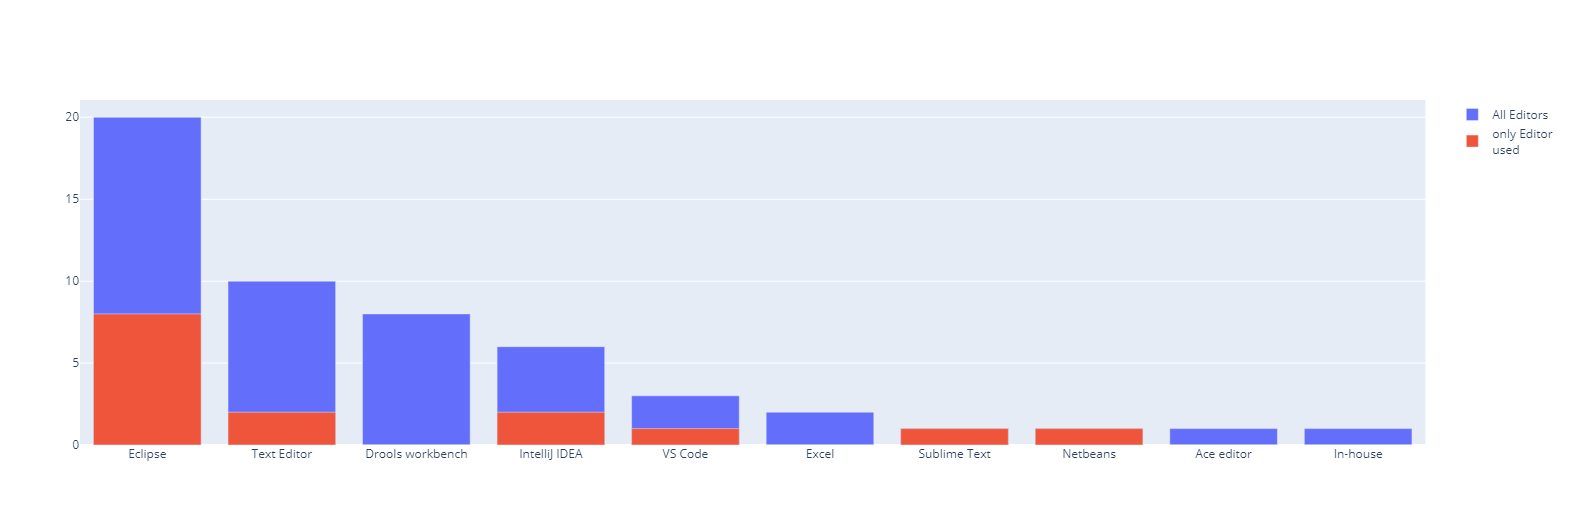
\includegraphics[width=0.95\textwidth]{Sections/images/EditorUseage.png}}
    \caption{Editors used}
    \label{fig:editorUsage}
\end{figure}


\subsection{Question Analysis}

\subsubsection{Grouping}
When displaying subtypes we shall split into groups.
The source of the response will create a pseudo cross-section of our participants.
The 10 who were contacted through academic papers will be considered our academics.
The remaining 20 will be considered practitioners.

The next grouping will be on Drools Experience.
The 9 who replied they had used drools ``for years and intensely'' are categorised as experts.
The 16 who either answered ``for years, but occasionally'' or ``not for long, but intensely'' are categorised as seniors.
The 5 who answered ``I barely touched it'' are categorised as novices.

Another grouping will be on recency of use.
The 12 who have used Drools in 2021 will be categorised as current users.
The remaining 18 as past users.

To remove some bias in the questionnaires we changed question order, order of projections, and which rulesets were used.
When a question is effected by this, then this will also be displayed.

\subsubsection{Display}
Until now, the choice of chart to display the survey outcome has been based on a feeling rather than research. 
For the remainder of this section we will rely on the advice of our predecessors.

The remainder of this Results sections, whilst displaying results that regard our Likert scaled questions, we will be following the advice of Robbins et.al.\cite{robbins2011plotting} by using diverging stacked bar charts, with counts added.
This style allows the evaluation of subclasses results.
The addition of counts makes it easier to spot when the results are skewed by small numbers.

In our charts we will take positive scores as being right of the center line and neutral and negative scores as being left.
With our particular question design, we are unable to tell if the neutral responses are substantive or hidden non responses\cite{blasius2001use}.
% We, rather arbitrarily decided, in a similar fashion to the Net Promoter Score\cite{reichheld2003one} (NPS), to include the middle results as being negative.

\subsubsection{Grouping Analysis}
Our data does not fall under a normal distribution, so we will be using a nonparametric test.
Vaus\cite{de2013surveys} advises that when analysing Ordinal variables with nominal grouping variables then the statistical methods one should use for checking for differences between groupings would be the Mann-Whitney\cite{mann1947test} or the Kruskal Wallis\cite{kruskal1952use} tests.
In the grouping section we had one group of only 5 participants, the novices.
As this group is too small to think of using in analysis we will ignore it.
This means that all of the groupings we have will be divided in two.
As Mann-Whitney is a specialisation of Kruskal Wallis for two groups, this is the analysis we will use.

For all our analyizes our null hypothesis, H\textsubscript{0}, is that there is no between the ranks of the two groups. 
Our alternative hypothesis, H\textsubscript{1}, is there is a difference between the ranks of the two groups.
Our alpha, or significance, level will be 0.05, for no other reason than it seems to be a mutually agreed upon value within the statistical community, and justifying a different significance would take more time than is warranted for the value these analysizes will give.
Our sample size is greater than 20, thus we can use a Z distribution.

To work out out Z score, we have an alpha level of 0.05 and a 2 tailed test.
We could work the distribution out by using the following formula:
\[U_{1}=n_{1}n_{2}+\frac{n_{1}(n_{1}+1)}{2}-R_{1}\]
However it is easier to look up in a Z table.
Thus, we have an area in body of 0.9750, which correlates in the Z Table to a z value of 1.96.
Thus our decision rule is, If our z is less than -1.96, or greater than 1.96, we reject our null hypothesis.
\footnote{We carried out the calculations using the Mann-Whitney U Test calculator at \url{https://www.socscistatistics.com/tests/mannwhitney/default2.aspx}}

\pagebreak
\subsubsection{Question 1, 2 and 3: First Impressions}

\begin{figure}[h]
    \centering
    \fbox{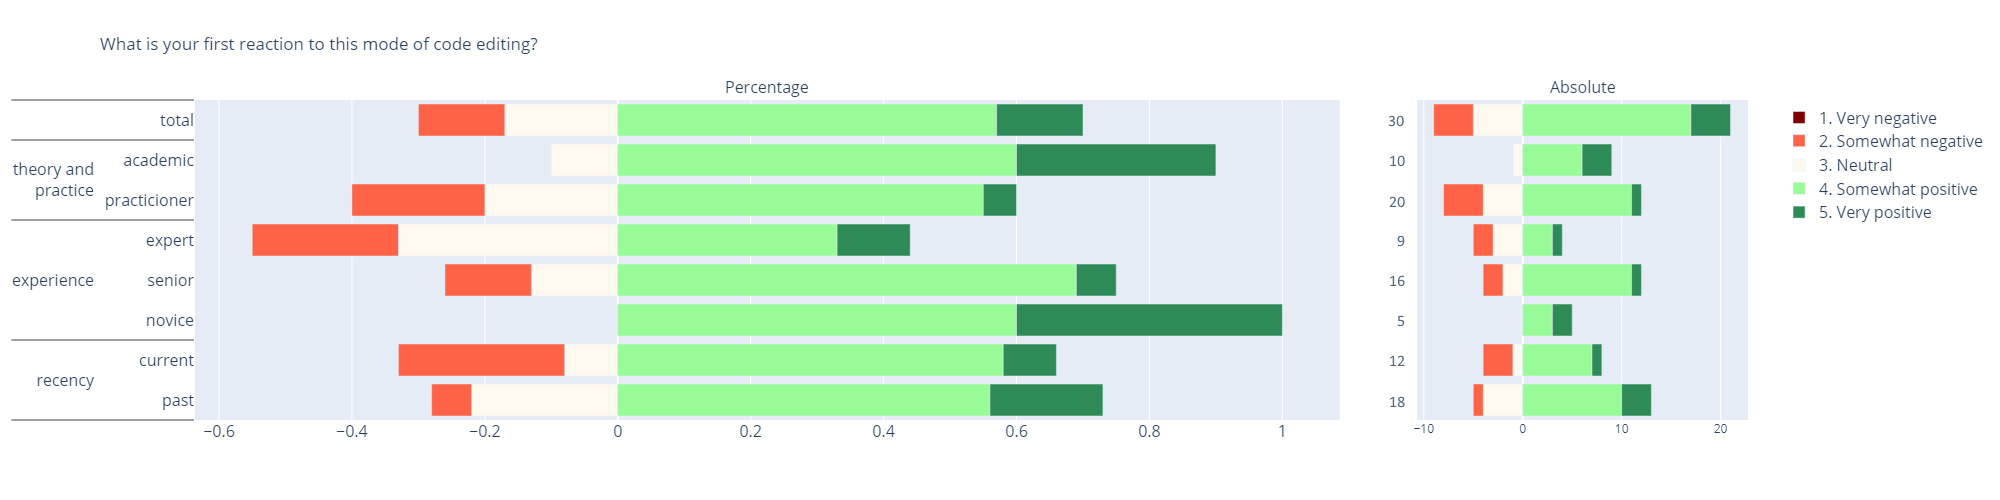
\includegraphics[width=0.95\textwidth]{Sections/images/stackedbar_Q1.png}}
    \caption{Question 1 - first impressions}
    \label{fig:stackedbar_Q1}
\end{figure}

\begin{table}[h]
    \begin{center}
        \begin{tabular}{ |l ||r |r |r | r|l | } 
            \hline
            Group Comparison                 & Critical U & U-value & z-Score  & p-value & Hypothesis         \\
            \hline
            \hline
            Academic vs Practitioner         & 55         & 54.5    & -1.97974 & 0.0477  & \textbf{H\textsubscript{1}}  \\ 
            \hline
            Expert vs Senior                 & 37         & 55      & 0.93413  & 0.35238 & H\textsubscript{0} \\ 
            \hline
            Current vs Past                  & 61         & 91      & 0.6985   & 0.48392 & H\textsubscript{0} \\ 
            \hline
        \end{tabular}
    \end{center}
    \caption{Mann-Whitney question 1 - first impressions}
    \label{table:mannwhitneyQ1}
\end{table}

This question shows the subject an example of projectional editing a Drools file alongside a table projection, as an animated GIF, along with an explanation.
Then she is asked her first reaction. 
The chart in figure \ref{fig:stackedbar_Q1} shows the outcomes.
Eyeballing the chart, an observation that can be taken is that the novice and the academics (where there is a lot of crossover), found the initial presentation more positive than the experienced practitioners.

Table \ref{table:mannwhitneyQ1}, shows that there is a significant difference between how academics and practitioners first react to seeing the projectional editing example.
Here, the academics have a far more positive view of the example than the practitioners.

In general, we see an overwhelmingly positive response.
There were 5 times as many positive (21) then negative (4) responses.
Those who had a positive or negative responses were directed to answer the open questions ``Q2. How would this coding style be useful to your interactions with Drools?'' and ``Q3. What do you find negative with this style of coding?'' respectively.
Figure \ref{fig:wordclouds} show a not very useful, but funky looking visualization of the subjects responses.

\begin{figure}[H]
    \begin{subfigure}{.60\textwidth}
      \centering
      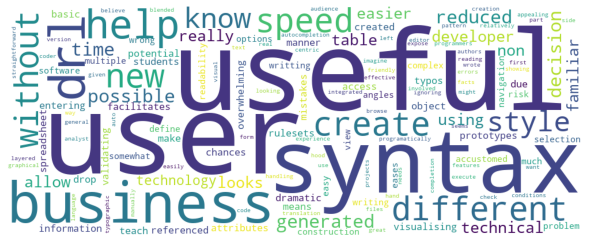
\includegraphics[width=.95\linewidth]{Sections/images/positive_wordcloud.png}
      \caption{Positive}
      \label{fig:wfig1}
    \end{subfigure}%
    \begin{subfigure}{.40\textwidth}
      \centering
      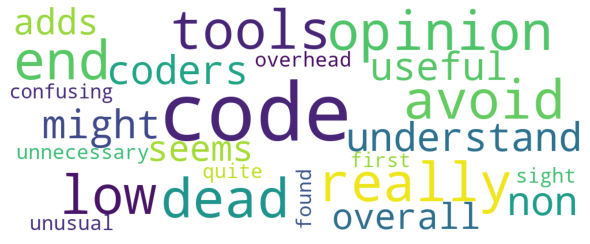
\includegraphics[width=.95\linewidth]{Sections/images/negative_wordcloud.png}
      \caption{Negative}
      \label{fig:wfig2}
    \end{subfigure}
    \caption{Initial thoughts}
    \label{fig:wordclouds}
\end{figure}

Amongst the positive comments it appears the the subjects had all picked up on many of the advantages that projectional editing brings.
The ones that got the most mentions, using other words, were exploratory coding, correctness by construction, and multiple viewpoints.
It was also noted, with the projections shown, that development could be quicker and easier to check.

Amongst the, very few, negative comments, they discussed the failures of no/low code solutions, that the view was confusing and they felt it added unnecessary overhead.

\subsubsection{Question 4 and 5: Interpret Projection}

\begin{figure}[H]
    \centering
    \fbox{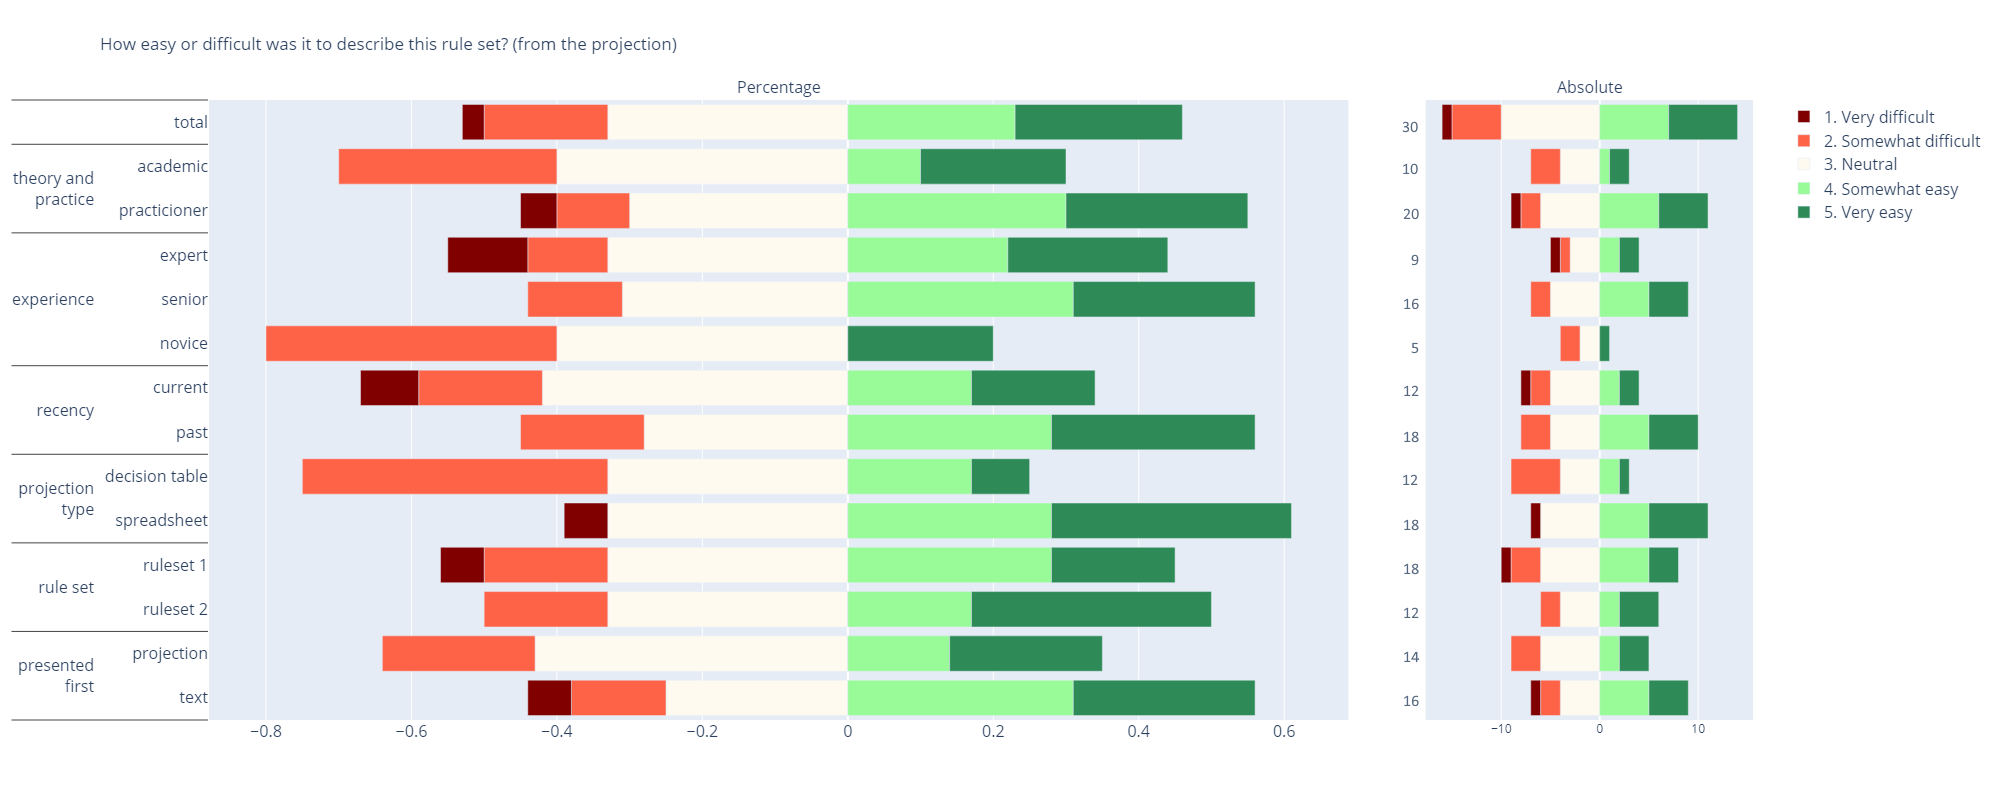
\includegraphics[width=0.95\textwidth]{Sections/images/stackedbar_Q2.png}}
    \caption{Question 5 - interpret projection}
    \label{fig:stackedbar_Q2}
\end{figure}

\begin{table}[H]
    \begin{center}
        \begin{tabular}{ |l ||r |r |r | r|l | } 
            \hline
            Group Comparison                 & Critical U & U-value & z-Score  & p-value & Hypothesis         \\
            \hline
            \hline
            Academic vs Practitioner         & 55        & 77      &  0.98987  & 0.32218 & H\textsubscript{0} \\ 
            \hline
            Expert vs Senior                 & 37        & 61.5    &  0.56614  & 0.56868 & H\textsubscript{0} \\ 
            \hline
            Current vs Past                  & 61        & 82.5    &  1.05833  & 0.28914 & H\textsubscript{0} \\ 
            \hline
            Decision Table vs Spreadsheet    & 55        & 61      &  2.2225   & 0.02642 & \textbf{H\textsubscript{1}}  \\ 
            \hline
            Ruleset 1 vs Ruleset 2           & 61        & 92      &  0.65617  & 0.50926 & H\textsubscript{0} \\ 
            \hline
            Projection first vs Text first   & 64        & 97      &  0.60277  & 0.5485  & H\textsubscript{0} \\ 
            \hline
        \end{tabular}
    \end{center}
    \caption{Mann-Whitney question 5 - interpret projection}
    \label{table:mannwhitneyQ2}
\end{table}

This question asks the subject to describe the meaning of the projection and then describe how hard it was to do that.
Very few people described the meaning of the projection well.

The chart in figure \ref{fig:stackedbar_Q2} shows the outcomes.
Looking at the chart, it appears obvious that there is a difference in confidence of the subjects between the different projections presented.
The participants believed they understood the spread sheet style projection better then the decision table projection.

This observation is confirmed in the Mann-Whitney analysis, shown in table \ref{table:mannwhitneyQ2}.
Otherwise, no other grouping differed significantly from the general population.

The ratio of those thinking it was easy to those thinking it was hard to understand the projection was ~2:1, 14 to 6.

There was one extreme response, which was negative.
This came from an expert practitioner who saw the text version before seeing the projection.

\subsubsection{Question 6 and 7: Interpret Text}

\begin{figure}[H]
    \centering
    \fbox{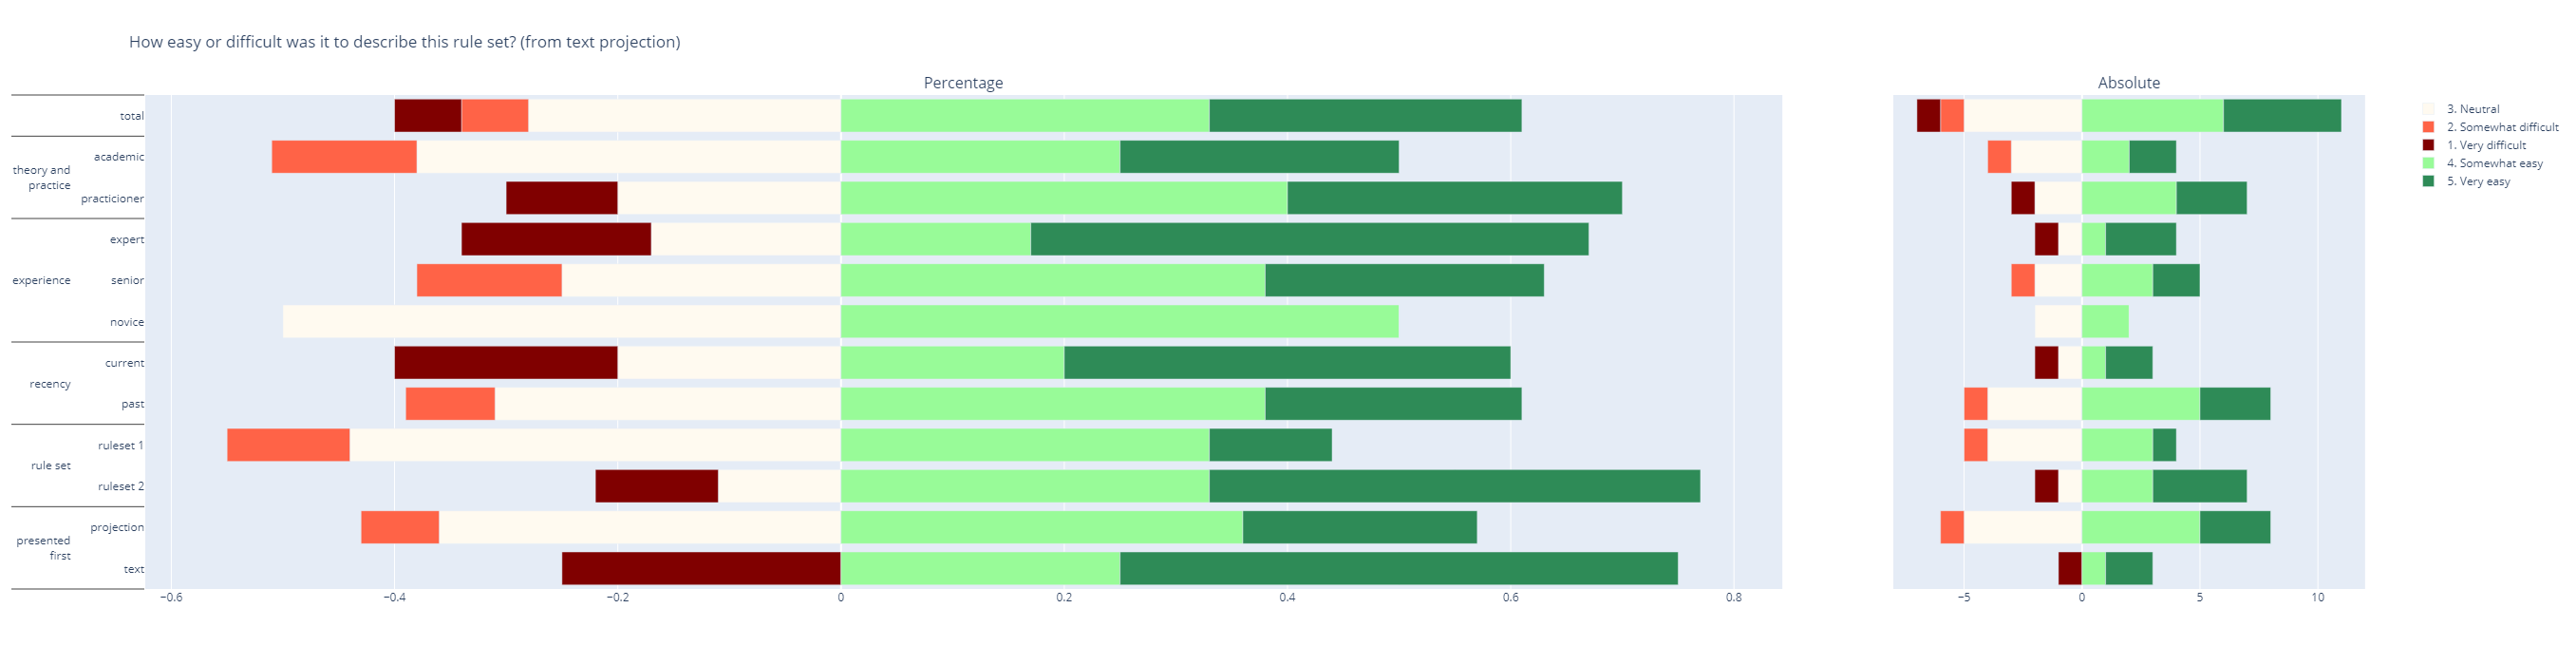
\includegraphics[width=0.95\textwidth]{Sections/images/stackedbar_Q3.png}}
    \caption{Question 7 - interpret text}
    \label{fig:stackedbar_Q3}
\end{figure}

\begin{table}[H]
    \begin{center}
        \begin{tabular}{ |l ||r |r |r | r|l | } 
            \hline
            Group Comparison                 & Critical U & U-value & z-Score  & p-value & Hypothesis         \\
            \hline
            \hline
            Academic vs Practitioner         & 17         & 34      &  0.48869 & 0.62414 & H\textsubscript{0} \\ 
            \hline
            Expert vs Senior                 & 8          & 20.5    &  -0.3873 & 0.69654 & H\textsubscript{0} \\ 
            \hline
            Current vs Past                  & 12         & 31.5    &  -0.04929& 0.96012 & H\textsubscript{0} \\ 
            \hline
            Ruleset 1 vs Ruleset 2           & 17         & 24.5    &  -1.36868& 0.17068 & H\textsubscript{0} \\ 
            \hline
        \end{tabular}
    \end{center}
    \caption{Mann-Whitney question 7 - interpret text}
    \label{table:mannwhitneyQ3}
\end{table}

This question asks the subject to interpret a rule set that is presented in a Drools style text projection.
The purpose of this question was three fold.
First, to calibrate how well the subject really understood drools.
Second, for a comparison with with a later projection.
Finally, to calibrate whether and how much easier the text was than the projection to those used to seeing the text version.

Unfortunately, we assume due to the questionnaire design, there was a large number of non-respondents to this question. 
12 of the 30 respondents did not answer this question.
All 12 of these were from the 16 that were presented the text projection before the tabular projections.

Reporting on 18 responses has a lot less validity.
With that in mind in figure \ref{fig:stackedbar_Q3}, we can see a much higher confidence in the easiness of understanding the rule set.
We see a 5:1 ratio of greater belief in the participants that it was easy to understood the meaning of the text projections.
This proportion is significantly higher than those who thought it was easy to understood the tabular projections.

The Mann-Whitney table does not show any significant differences in any of the groups.
We are unable to report on the difference between those who were presented the text projection first or the tabular projection first.
The 4 participants responding from the group who were presented text first, was too low to give a meaningful score.

\pagebreak
\subsubsection{Question 8: Compare Projections}

\begin{figure}[H]
    \centering
    \fbox{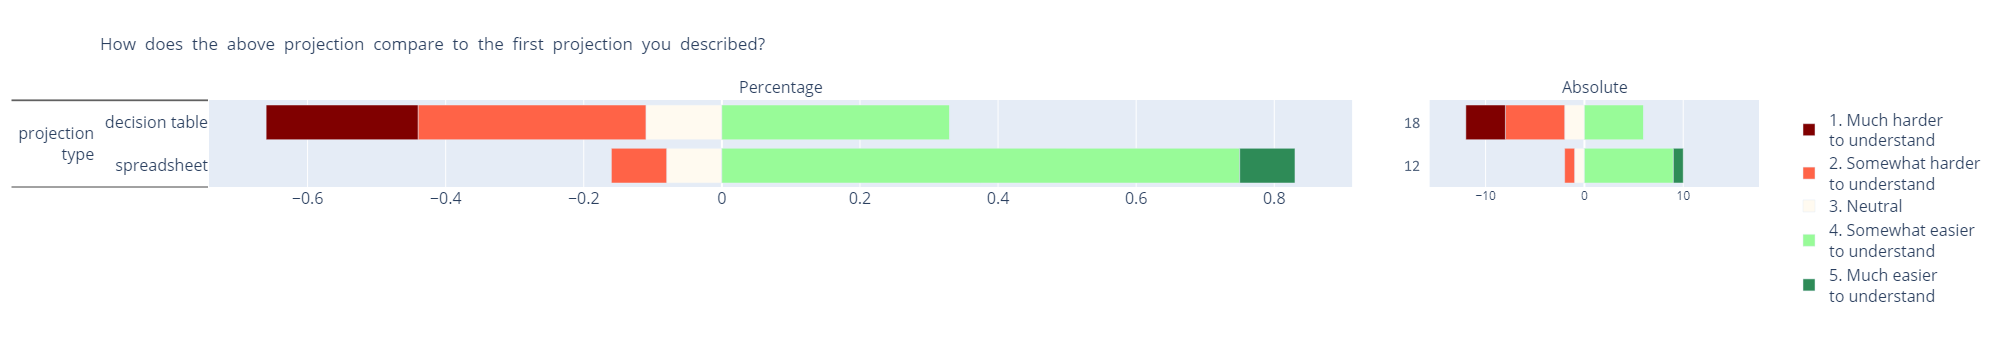
\includegraphics[width=0.95\textwidth]{Sections/images/stackedbar_Q4a.png}}
    \caption{Question 8 - compare projections}
    \label{fig:stackedbar_Q4}
\end{figure}

\begin{table}[H]
    \begin{center}
        \begin{tabular}{ |l ||r |r |r | r|l | } 
            \hline
            Group Comparison                 & Critical U & U-value & z-Score  & p-value & Hypothesis         \\
            \hline
            \hline
            Decision Table vs Spreadsheet    & 61         & 45      &  -2.64584& 0.00804 & \textbf{H\textsubscript{1}} \\ 
            \hline
        \end{tabular}
    \end{center}
    \caption{Mann-Whitney question 8 - compare projections}
    \label{table:mannwhitneyQ4}
\end{table}

This question asked the participant to compare the two tabular projections.  
This question was to calibrate whether one projection was considerably worse than the other and whether that would affect the comparison with text.

Looking the chart in figure \ref{fig:stackedbar_Q4}, we have ignored all bars except the difference between the projections presented.
The way the question is constructed the other groupings do not help.

It is obvious in this chart and confirmed in the Mann-Whitney analysis shown in table \ref{table:mannwhitneyQ4}, that the spreadsheet presentation is considered far easier to understand than the decision table.
This result correlates well with the difference in understanding found previously in question 5.

\subsubsection{Question 9: Compare Projection to Text}

\begin{figure}[H]
    \centering
    \fbox{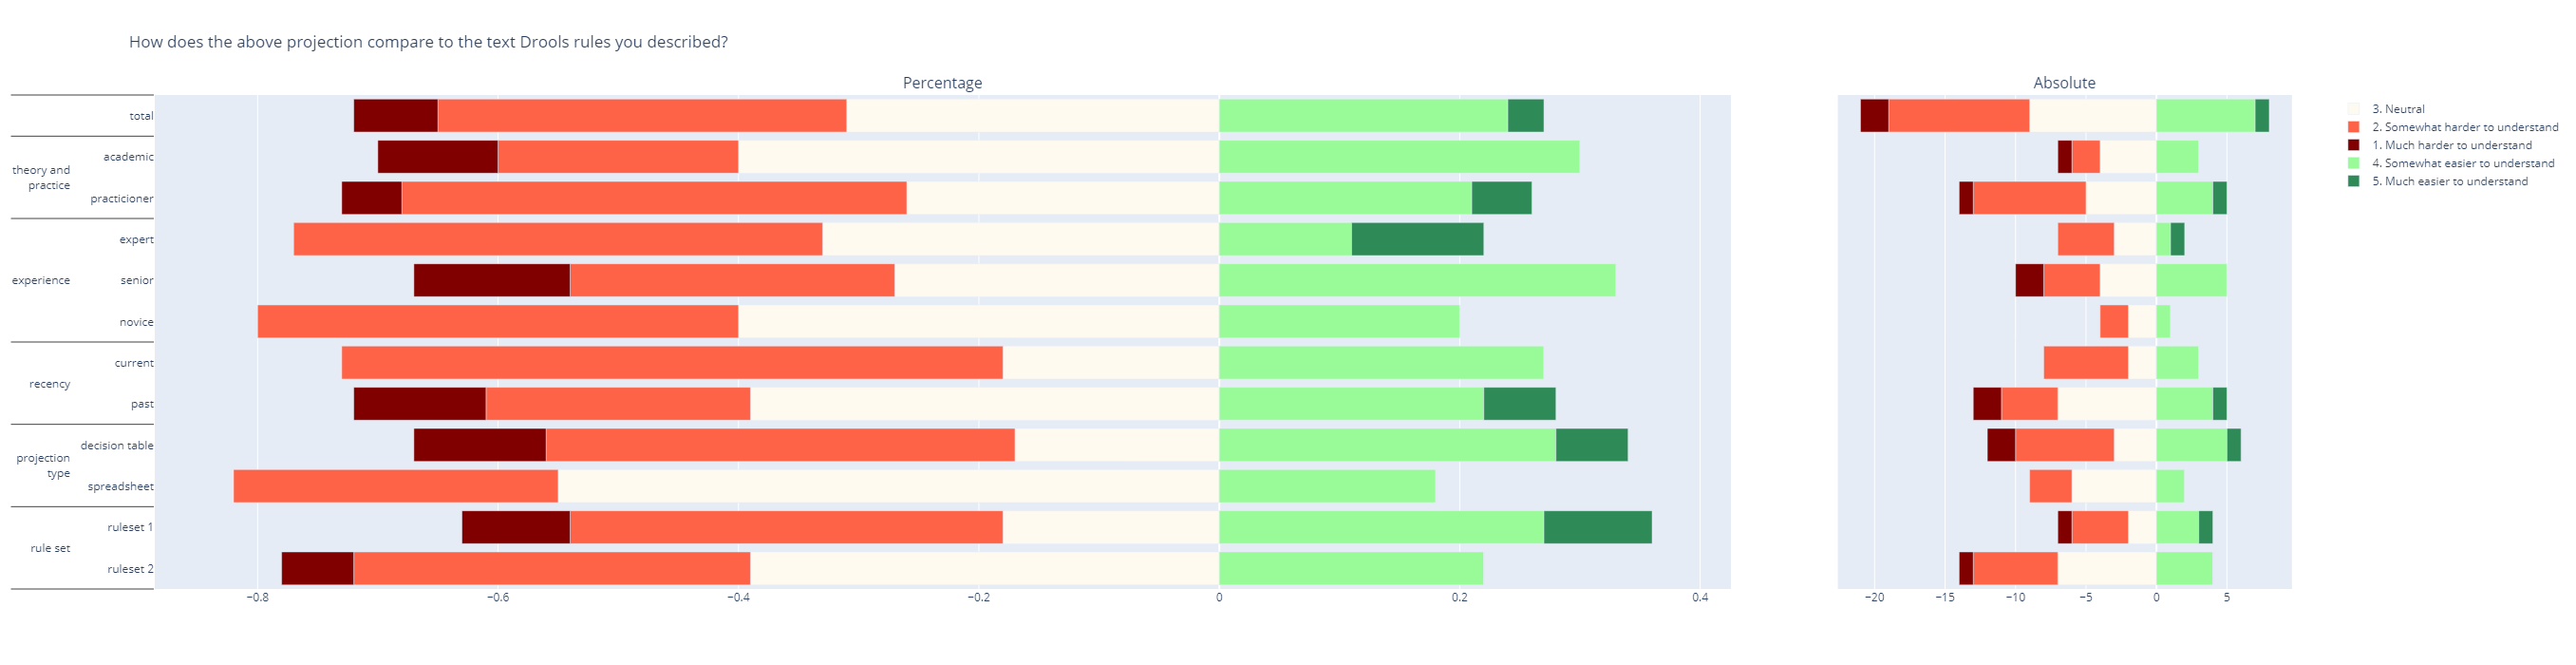
\includegraphics[width=0.95\textwidth]{Sections/images/stackedbar_Q5.png}}
    \caption{Question 9 - compare projections with text}
    \label{fig:stackedbar_Q5}
\end{figure}

\begin{table}[H]
    \begin{center}
        \begin{tabular}{ |l ||r |r |r | r|l | } 
            \hline
            Group Comparison                 & Critical U & U-value & z-Score  & p-value & Hypothesis         \\
            \hline
            \hline
            Academic vs Practitioner         & 52         & 85.5    & -0.41295 & 0.6818  & H\textsubscript{0} \\ 
            \hline
            Expert vs Senior                 & 34         & 67.5    & 0.02981  & 0.97606 & H\textsubscript{0} \\ 
            \hline
            Current vs Past                  & 55         & 88      & 0.47194  & 0.63836 & H\textsubscript{0} \\ 
            \hline
            Decision Table vs Spreadsheet    & 55         & 89.5    & -0.40452 & 0.68916 & H\textsubscript{0} \\ 
            \hline
            Ruleset 1 vs Ruleset 2           & 55         & 94.5    & -0.17979 & 0.85716 & H\textsubscript{0} \\ 
            \hline
        \end{tabular}
    \end{center}
    \caption{Mann-Whitney Question 9 - compare projections with text}
    \label{table:mannwhitneyQ5}
\end{table}

This question asked our subjects to compare a tabular projection with the text projection.
There was one participant that chose not to answer this question.

This result, shown in figure \ref{fig:stackedbar_Q5}, was pretty definitive.
The subjects found very much that the textual projections were more understandable than the tabular projections.
The ratio of harder to easier to understand was 3:2, with 12 subjects finding the Text projection easier to understand and 8 finding the projection easier.
Table \ref{table:mannwhitneyQ5} shows this was independent of any other factors.

\subsubsection{Question 10: Truth Table Validation}

\begin{figure}[H]
    \centering
    \fbox{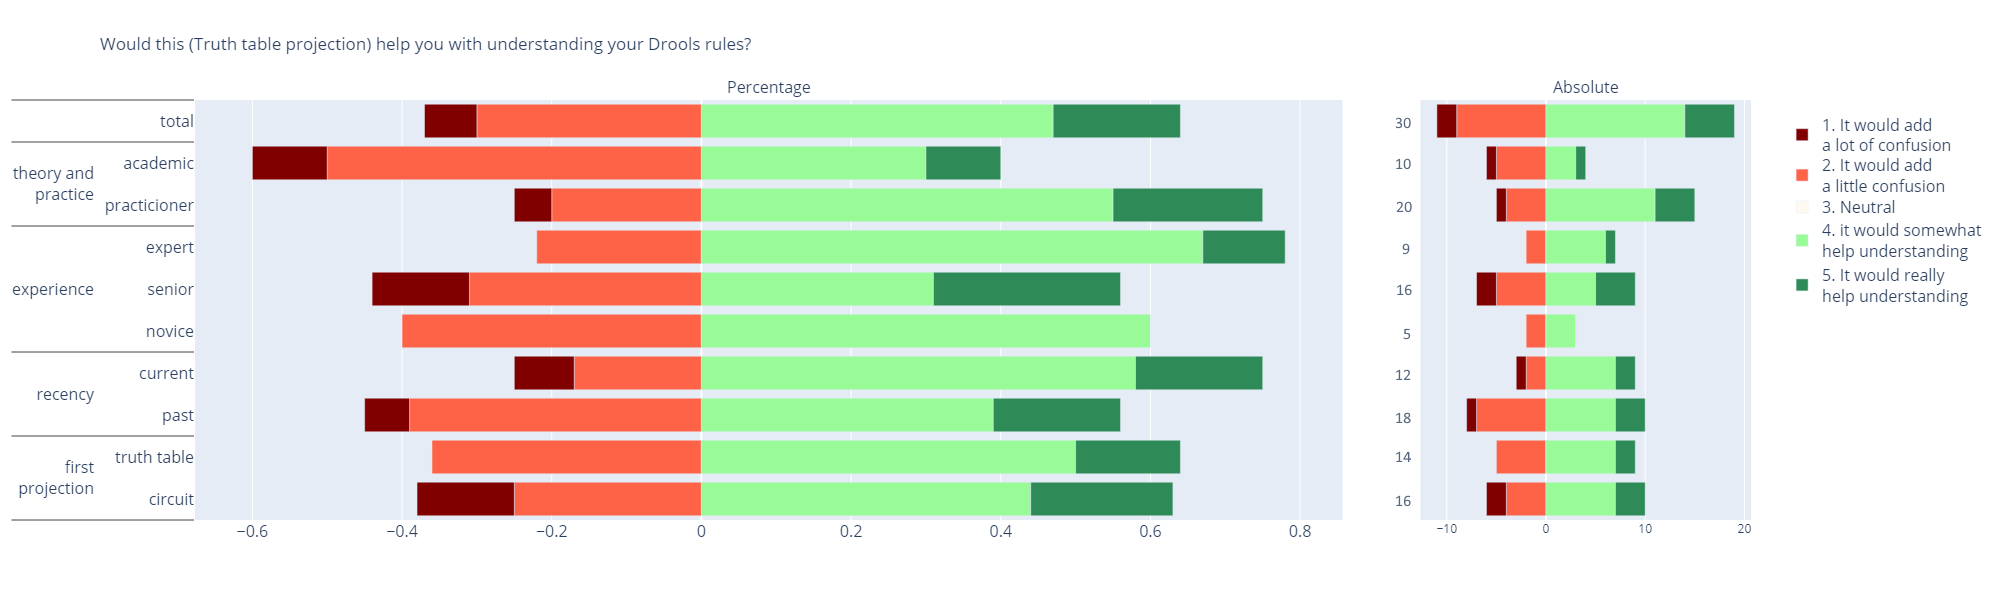
\includegraphics[width=0.95\textwidth]{Sections/images/stackedbar_Q6.png}}
    \caption{Question 10 - truth table}
    \label{fig:stackedbar_Q6}
\end{figure}

\begin{table}[H]
    \begin{center}
        \begin{tabular}{ |l ||r |r |r | r|l | } 
            \hline
            Group Comparison                   & Critical U & U-value & z-Score  & p-value & Hypothesis         \\
            \hline
            \hline
            Academic vs Practitioner           &  55        & 65      & 1.5178   & 0.12852 & H\textsubscript{0} \\ 
            \hline
            Expert vs Senior                   &  37        & 64      & -0.4246  & 0.67448 & H\textsubscript{0} \\ 
            \hline
            Current vs Past                    &  61        & 93      & -0.61383 & 0.54186 & H\textsubscript{0} \\ 
            \hline
            Truth table first vs Circuit first &  64        & 108.5   & -0.12471 & 0.90448 & H\textsubscript{0} \\ 
            \hline
        \end{tabular}
    \end{center}
    \caption{Mann-Whitney Question 10 - truth table}
    \label{table:mannwhitneyQ6}
\end{table}

This question presented the subject with a wireframe of a truth table and asked if it would help them with understanding.

Every subject had a positive or negative view of the projection.
0 of the 30 subjects gave a neutral result.
We found this a very unlikely result.

There was a net positive view of this projection, with a little less than 2:1 finding it more helpful (19) than confusing (11).

On first view of the chart in figure \ref{fig:stackedbar_Q6}, it seems that academics have a much more negative view of this projection, and experts a more positive outlook.
However, when the figures are examined under Mann-Whitney, as seen in table \ref{table:mannwhitneyQ6}, these differences were not statistically significant.

\subsubsection{Question 11: Circuit Diagram Validation}

\begin{figure}[H]
    \centering
    \fbox{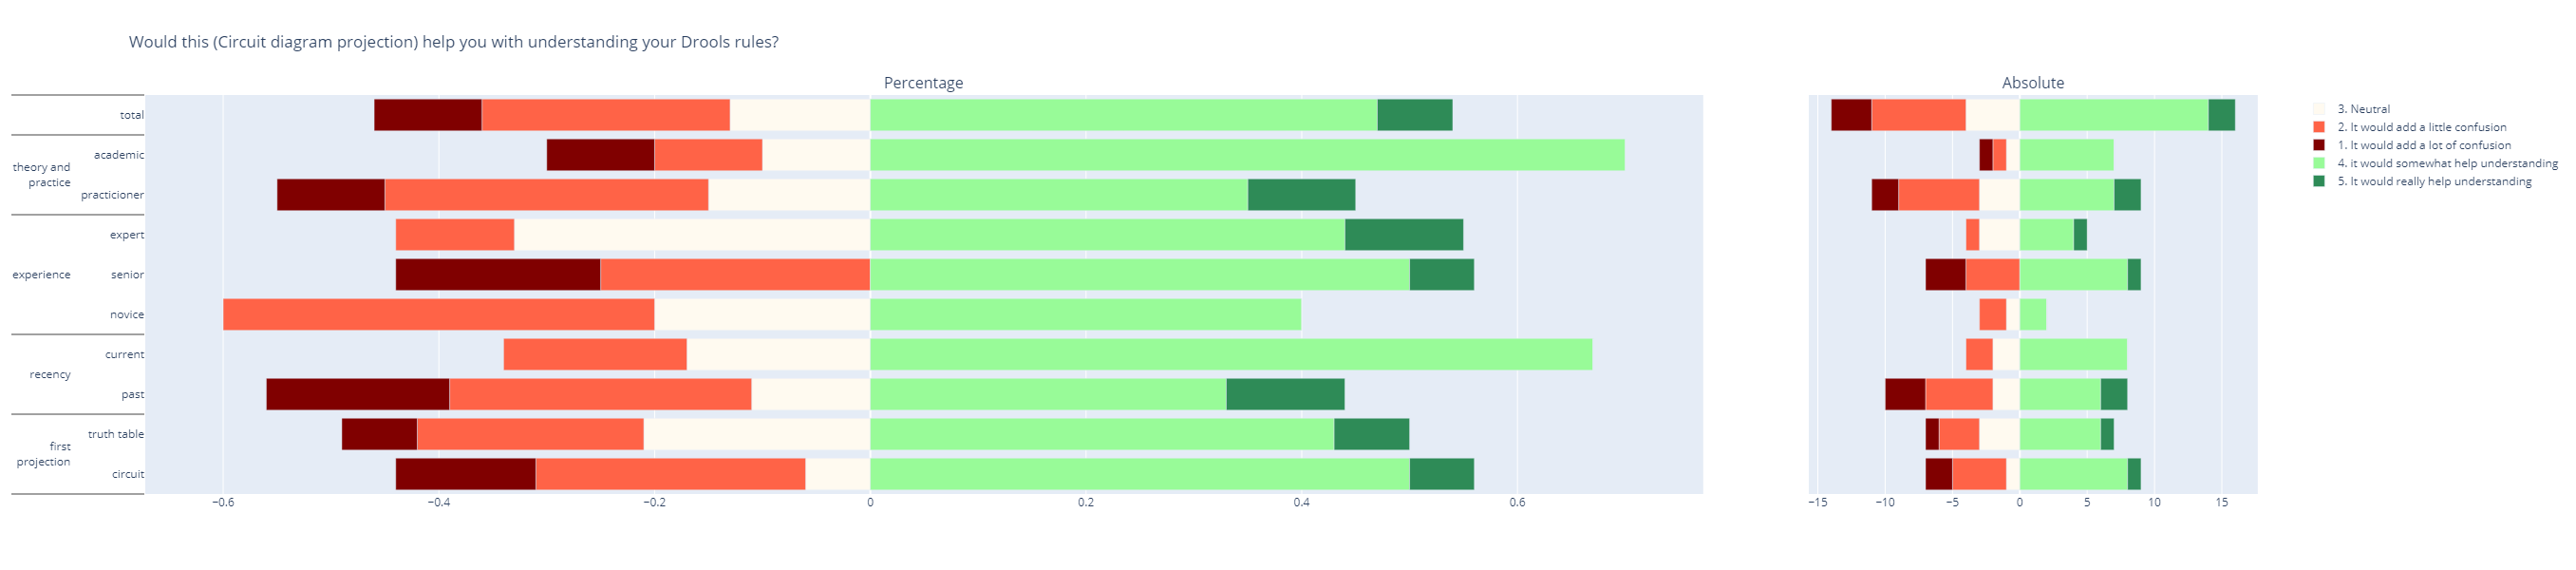
\includegraphics[width=0.95\textwidth]{Sections/images/stackedbar_Q7.png}}
    \caption{Question 11 - circuit diagram}
    \label{fig:stackedbar_Q7}
\end{figure}

\begin{table}[H]
    \begin{center}
        \begin{tabular}{ |l ||r |r |r | r|l | } 
            \hline
            Group Comparison                   & Critical U & U-value & z-Score  & p-value & Hypothesis         \\
            \hline
            \hline
            Academic vs Practitioner           & 55         & 83      & -0.7259  & 0.4654  & H\textsubscript{0} \\ 
            \hline
            Expert vs Senior                   & 37         & 58.5    & -0.73598 & 0.4593  & H\textsubscript{0} \\ 
            \hline
            Current vs Past                    & 61         & 83      & -1.03717 & 0.29834 & H\textsubscript{0} \\ 
            \hline
            Truth table first vs Circuit first & 64         & 110     & -0.06236 & 0.95216 & H\textsubscript{0} \\ 
            \hline
        \end{tabular}
    \end{center}
    \caption{Mann-Whitney Question 11 - circuit diagram}
    \label{table:mannwhitneyQ7}
\end{table}

This question presented the subject with a wireframe of a circuit diagram and asked if it would help them with understanding.

The view of the circuit diagram was a a net positive, with a ratio of ~ 3:2 (16 positive, 10 negative).

\subsubsection{Question 15: Closing Remarks}

Our last question asks for any last comments.
16 participants decided to add some words.

We ran sentiment analysis on these 16 comments, using the same service and similar code as we used in our SLR research, as described in section \ref{section:dataExtraction}.
9 were considered positive, 6 mixed and 1 negative.

Figure \ref{fig:Q15_wordcloud} shows a another pretty, but not too analytical word cloud.

The word that pops out, DMN, here is indicative of a few comments.
DMN is a tool for working with drools as a non developer.
There were some comments that our research should look in this direction.

The feeling was that the projections would give more advantage to non-developers.

There were some hints as to how to improve our projections or other projections to try.
Others suggested that the projections cannot capture some of the complexity of the rules that exist.

\begin{figure}[H]
    \centering
    \fbox{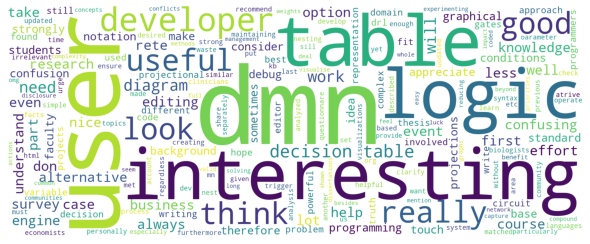
\includegraphics[width=0.95\textwidth]{Sections/images/Q15_wordcloud.png}}
    \caption{Question 15 - responses}
    \label{fig:Q15_wordcloud}
\end{figure}


\subsection{Summary Analysis}

The goal of this survey was to find if users of drools would find the projections we used useful.
The outcome seems to be yes, they seem useful, but not better than the text that they are currently used to.

We tried to control for different groupings that my effect the responses, and in most cases we found no significant differences in the groups we presented.

There was a significant difference between the projections presented, with the sample in general preferring the spreadsheet projection over the decision table. 
However, this was not what we were measuring for and even that is debatable as in question 9.
When comparing text to projection, the outcome for both tabular projections favoured text, but with a slightly lower net negative for the decision table comparison, 7:5 compared to 3:2.
